\subsection{HMBC}
\label{subsec:noah__hmbc}

The HMBC module is one which in fact does not fit perfectly into the NOAH principle of only exciting magnetisation which is needed.
As described in \cref{subsec:noah__case_studies}, the HMBC module should only require magnetisation of protons which have long-range couplings to \carbon{}; however, it ends up exciting \textit{all} \magnnot{C} magnetisation.
This leads to sharply reduced, and also unbalanced, intensities of homonuclear modules which come later in the supersequences.

I made some early (and brief) attempts at devising a pulse sequence which sought to discriminate these two magnetisation components using a perfect echo\autocite{Parella2019MRC}.
However, this was quickly abandoned as it proved very difficult to \textit{also} retain \magn{C} magnetisation.
I do not claim here that it is impossible to come up with a pulse sequence which does this, but it is certainly not easy, and ultimately I turned my focus to improving (rather than replacing) the HMBC module.


\subsubsection{Suppression of one-bond artefacts}

One of the issues with the NOAH HMBC module was that there were an unusual amount of one-bond artefacts, which arise from \magn{C} magnetisation which is allowed to evolve during the pulse sequence.
Generally, HMBC experiments seek to suppress this through the use of a low-pass J-filter (LPJF, see also \cref{subsec:poise__hmbc}).
The NOAH HMBC module \textit{additionally} contains a $zz$-filter, which stores \magn{C} magnetisation along $+z$ before the LPJF.
Thus, in theory, one-bond artefacts should be suppressed in the NOAH HMBC to an even greater extent.

However, this expectation is not borne out: in some cases, the NOAH HMBC in fact has \textit{more intense} one-bond artefacts when compared against a standard HMBC experiment (\cref{fig:noah_hmbc_1jch_no90,fig:noah_hmbc_1jch_std_lp2}).
Even performing an optimisation of the LPJF delays, as described in \cref{subsec:poise__hmbc}, did not lead to any reduction in artefacts.
I hypothesised instead that these artefacts arose from imperfect manipulation of \magn{C} magnetisation by the $zz$-filter.%
\footnote{It would be nice to back this up with simulations, but I did not have the time to run these.}
In particular, any \textit{antiphase} magnetisation (of the form $I_xS_z$ or $I_yS_z$) generated after the $zz$-filter would be reconverted into in-phase $I_x$ or $I_y$ terms, which would not be destroyed by the LPJF.
(The LPJF works based on the assumption that there is in-phase magnetisation at the beginning of it, which is true if the excitation element is just a \proton{} \ang{90} pulse.)

Such antiphase terms can be easily removed by the addition of a \carbon{} \ang{90} pulse, which transforms them into a mixture of double- and zero-quantum terms: these are either unobservable, or can be efficiently dephased by CTP gradients.
This technique is used in the CLIP-HSQC family of experiments\autocite{Enthart2008JMR,Gyongyosi2021AC}, as well as the LPJF itself.
In this case, we simply need to add an additional \carbon{} \ang{90} pulse at the end of the $zz$-filter: this pulse is highlighted in \cref{fig:noah_sb_po_b}.
This results in a striking reduction of the one-bond artefacts, as shown in \cref{fig:noah_hmbc_1jch_90}.
The suppression accomplished with the addition of this \ang{90} pulse is superior to that in the standard HMBC (\cref{fig:noah_hmbc_1jch_std_lp2}), and is comparable to a standard HMBC with a third-order LPJF (\cref{fig:noah_hmbc_1jch_std_lp3}).
Of course, the NOAH module---which by default uses a second-order LPJF---can also be `upgraded' to use a third-order LPJF.
In GENESIS pulse programmes, this can be done using the \texttt{-DLP3} acquisition flag (although the results were not evaluated here).

\begin{figure}[!ht]
    \centering
    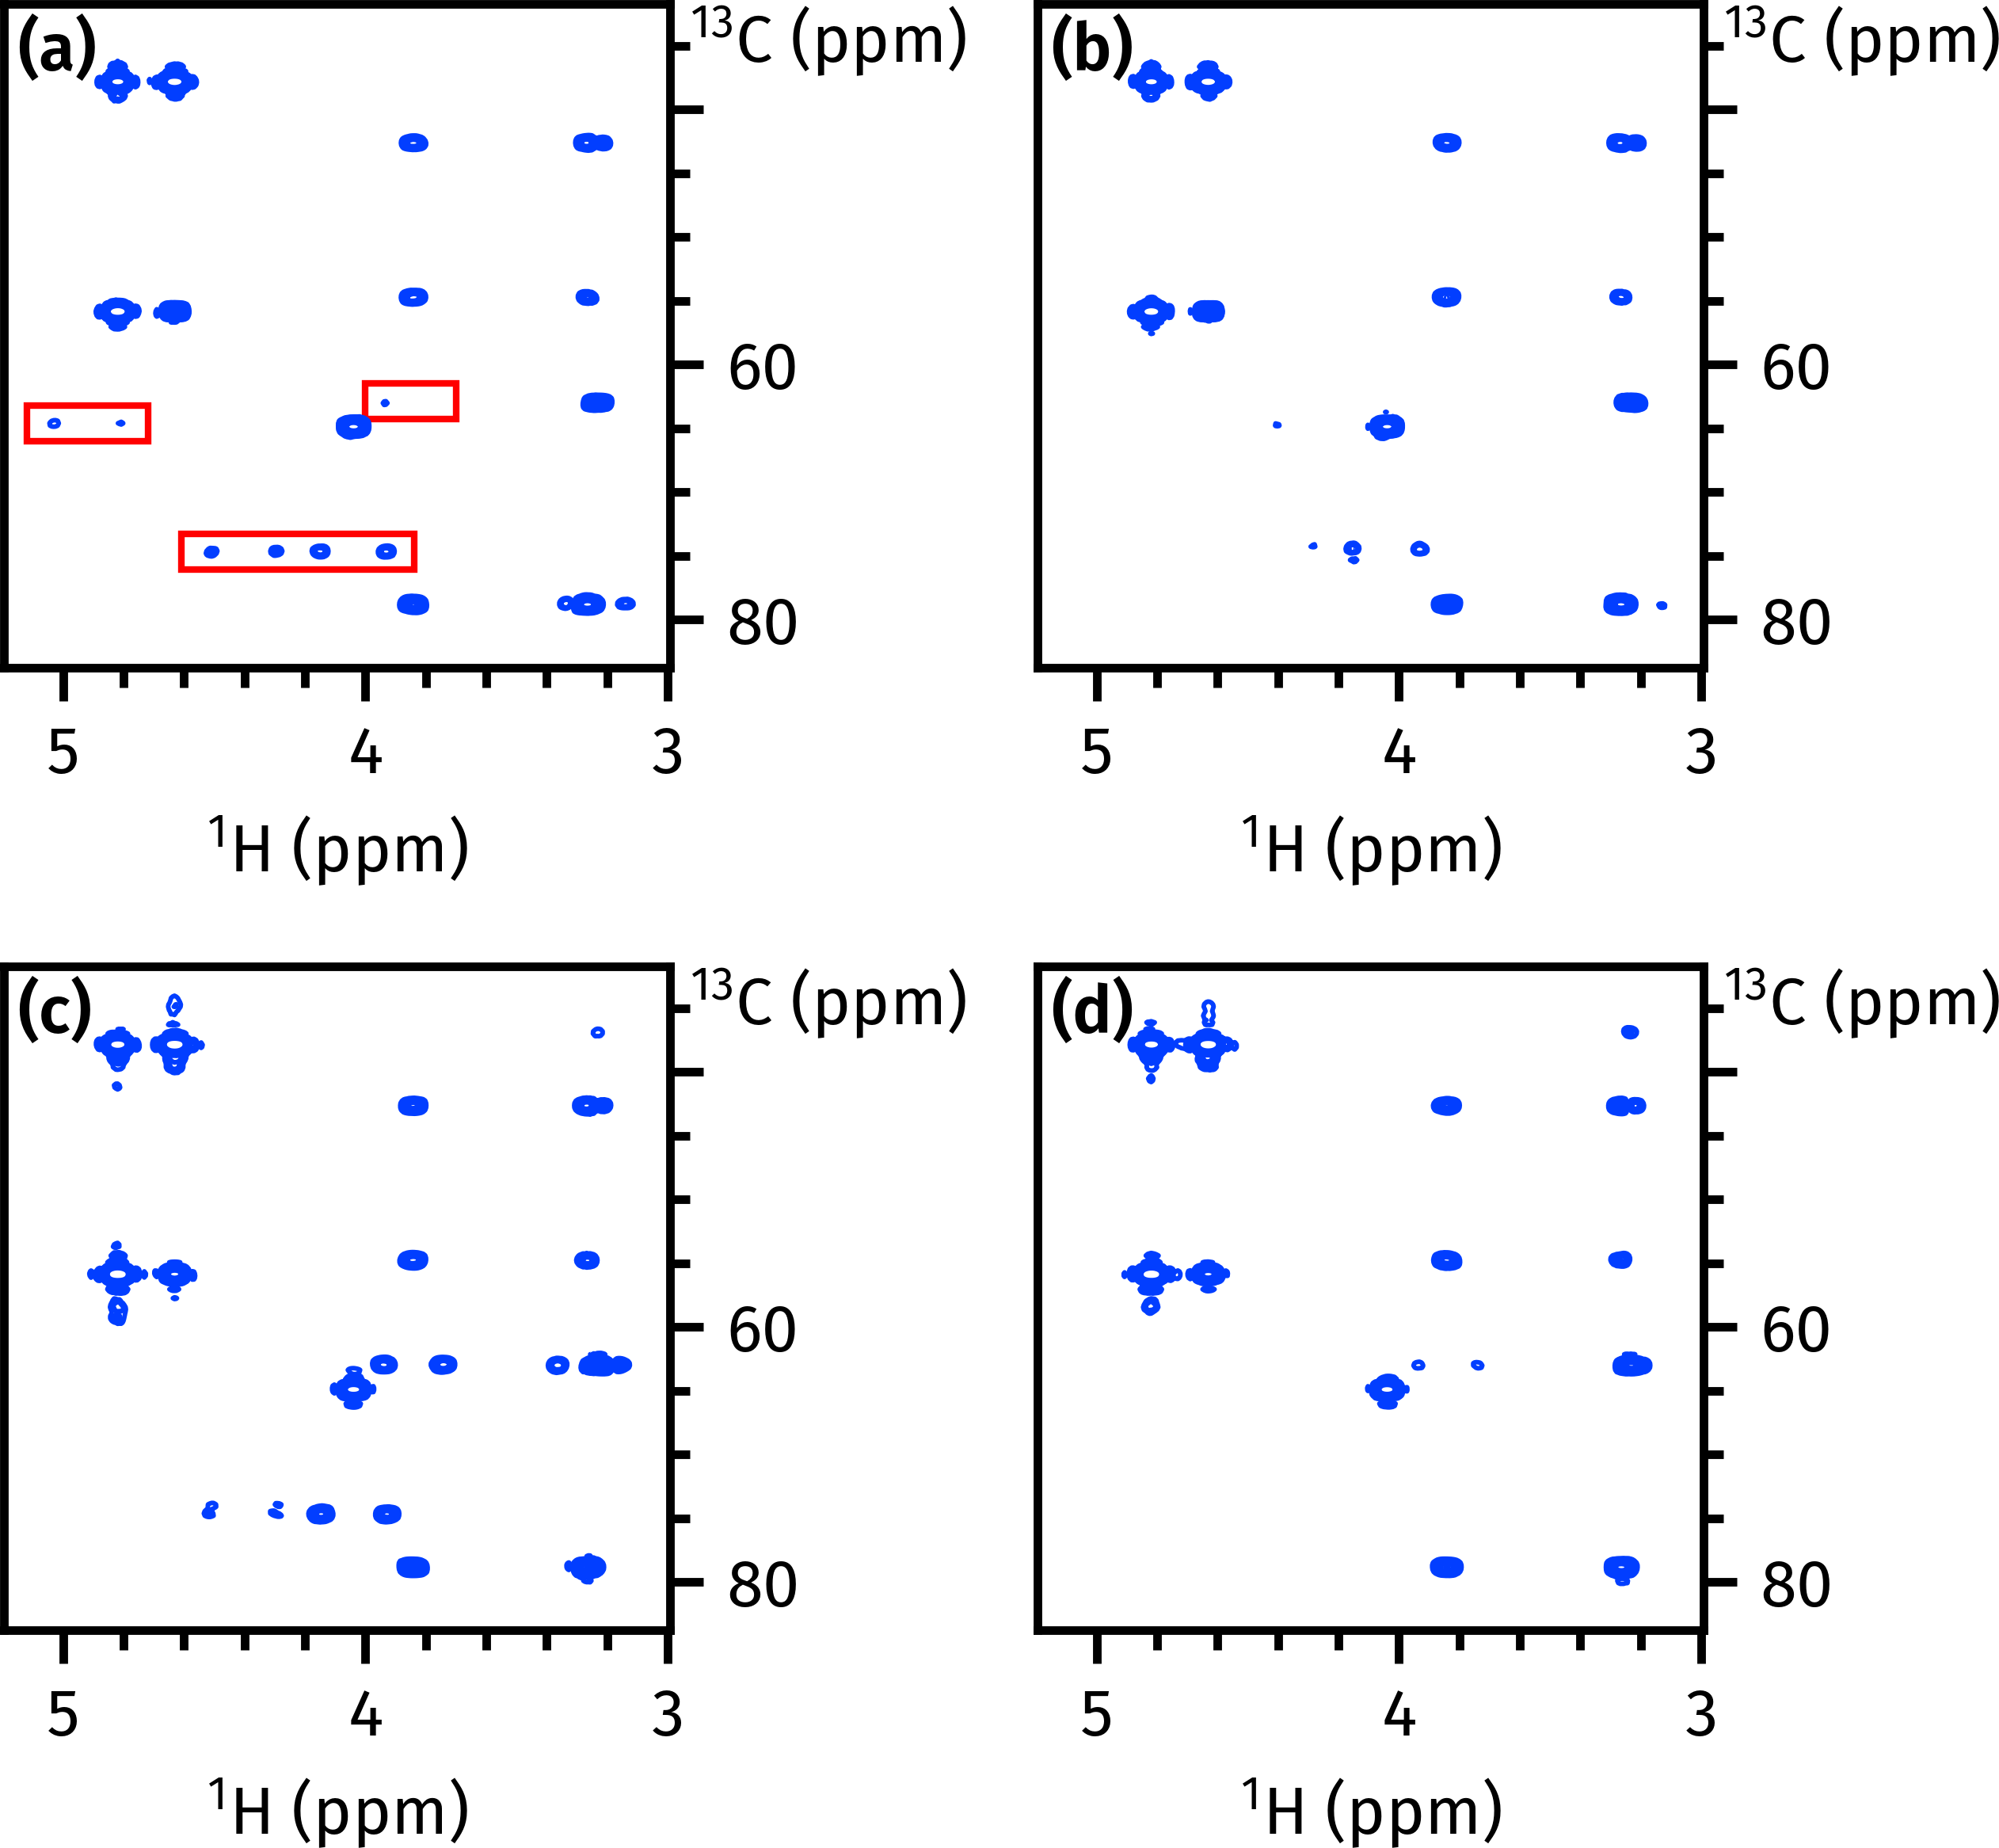
\includegraphics[]{noah/hmbc_1jch.png}%
    {\phantomsubcaption\label{fig:noah_hmbc_1jch_no90}}%
    {\phantomsubcaption\label{fig:noah_hmbc_1jch_90}}%
    {\phantomsubcaption\label{fig:noah_hmbc_1jch_std_lp2}}%
    {\phantomsubcaption\label{fig:noah_hmbc_1jch_std_lp3}}%
    \caption[Suppression of one-bond artefacts in NOAH HMBC spectra]{
        \textbf{(\subref{fig:noah_hmbc_1jch_no90})} NOAH $zz$-HMBC module without the additional \ang{90} pulse.
        One-bond artefacts are highlighted in red.
        \textbf{(\subref{fig:noah_hmbc_1jch_90})} NOAH $zz$-HMBC with the \ang{90} pulse.
        \textbf{(\subref{fig:noah_hmbc_1jch_std_lp2})} Standard library HMBC with a second-order LPJF.
        \textbf{(\subref{fig:noah_hmbc_1jch_std_lp3})} Standard library HMBC with a third-order LPJF.
        \datacode{7A-210916}
    }
    \label{fig:noah_hmbc_1jch}
\end{figure}


\subsubsection{Gradient selection schemes}

Another point which was investigated (but bore less fruit) was the gradient scheme used for CTP selection.
The NOAH module, as shown in \cref{fig:noah_sb_po_b}, uses a `symmetric' scheme where two gradients of equal amplitude surround the $t_1$ period: this encoding is later decoded by a third gradient just prior to acquisition.
However, other choices exist: for example, the Bruker standard library HMBC (derived from the work of Cicero et al.\autocite{Cicero2001JMR}) uses only two gradients in total, which have unequal amplitudes.

This gradient scheme cannot be directly used in a NOAH HMBC module, though.
This is because the $zz$-filter element places \magn{C} magnetisation along the $+z$ axis just before the HMBC J-evolution delay (see \cref{fig:noah_sb_po_b}).
This magnetisation later experiences the \proton{} \ang{180} pulse in the middle of $t_1$, which means that an extra \ang{180} pulse must be added at the very end of the sequence to finally return it to $+z$.
It is necessary to ensure that there is at least one gradient placed after this \ang{180} pulse to ensure proper CTP selection (in the `symmetric' scheme of \cref{fig:noah_sb_po_b}, this is fulfilled by the gradient $g_2$).

\begin{figure}[!htbp]
    \centering
    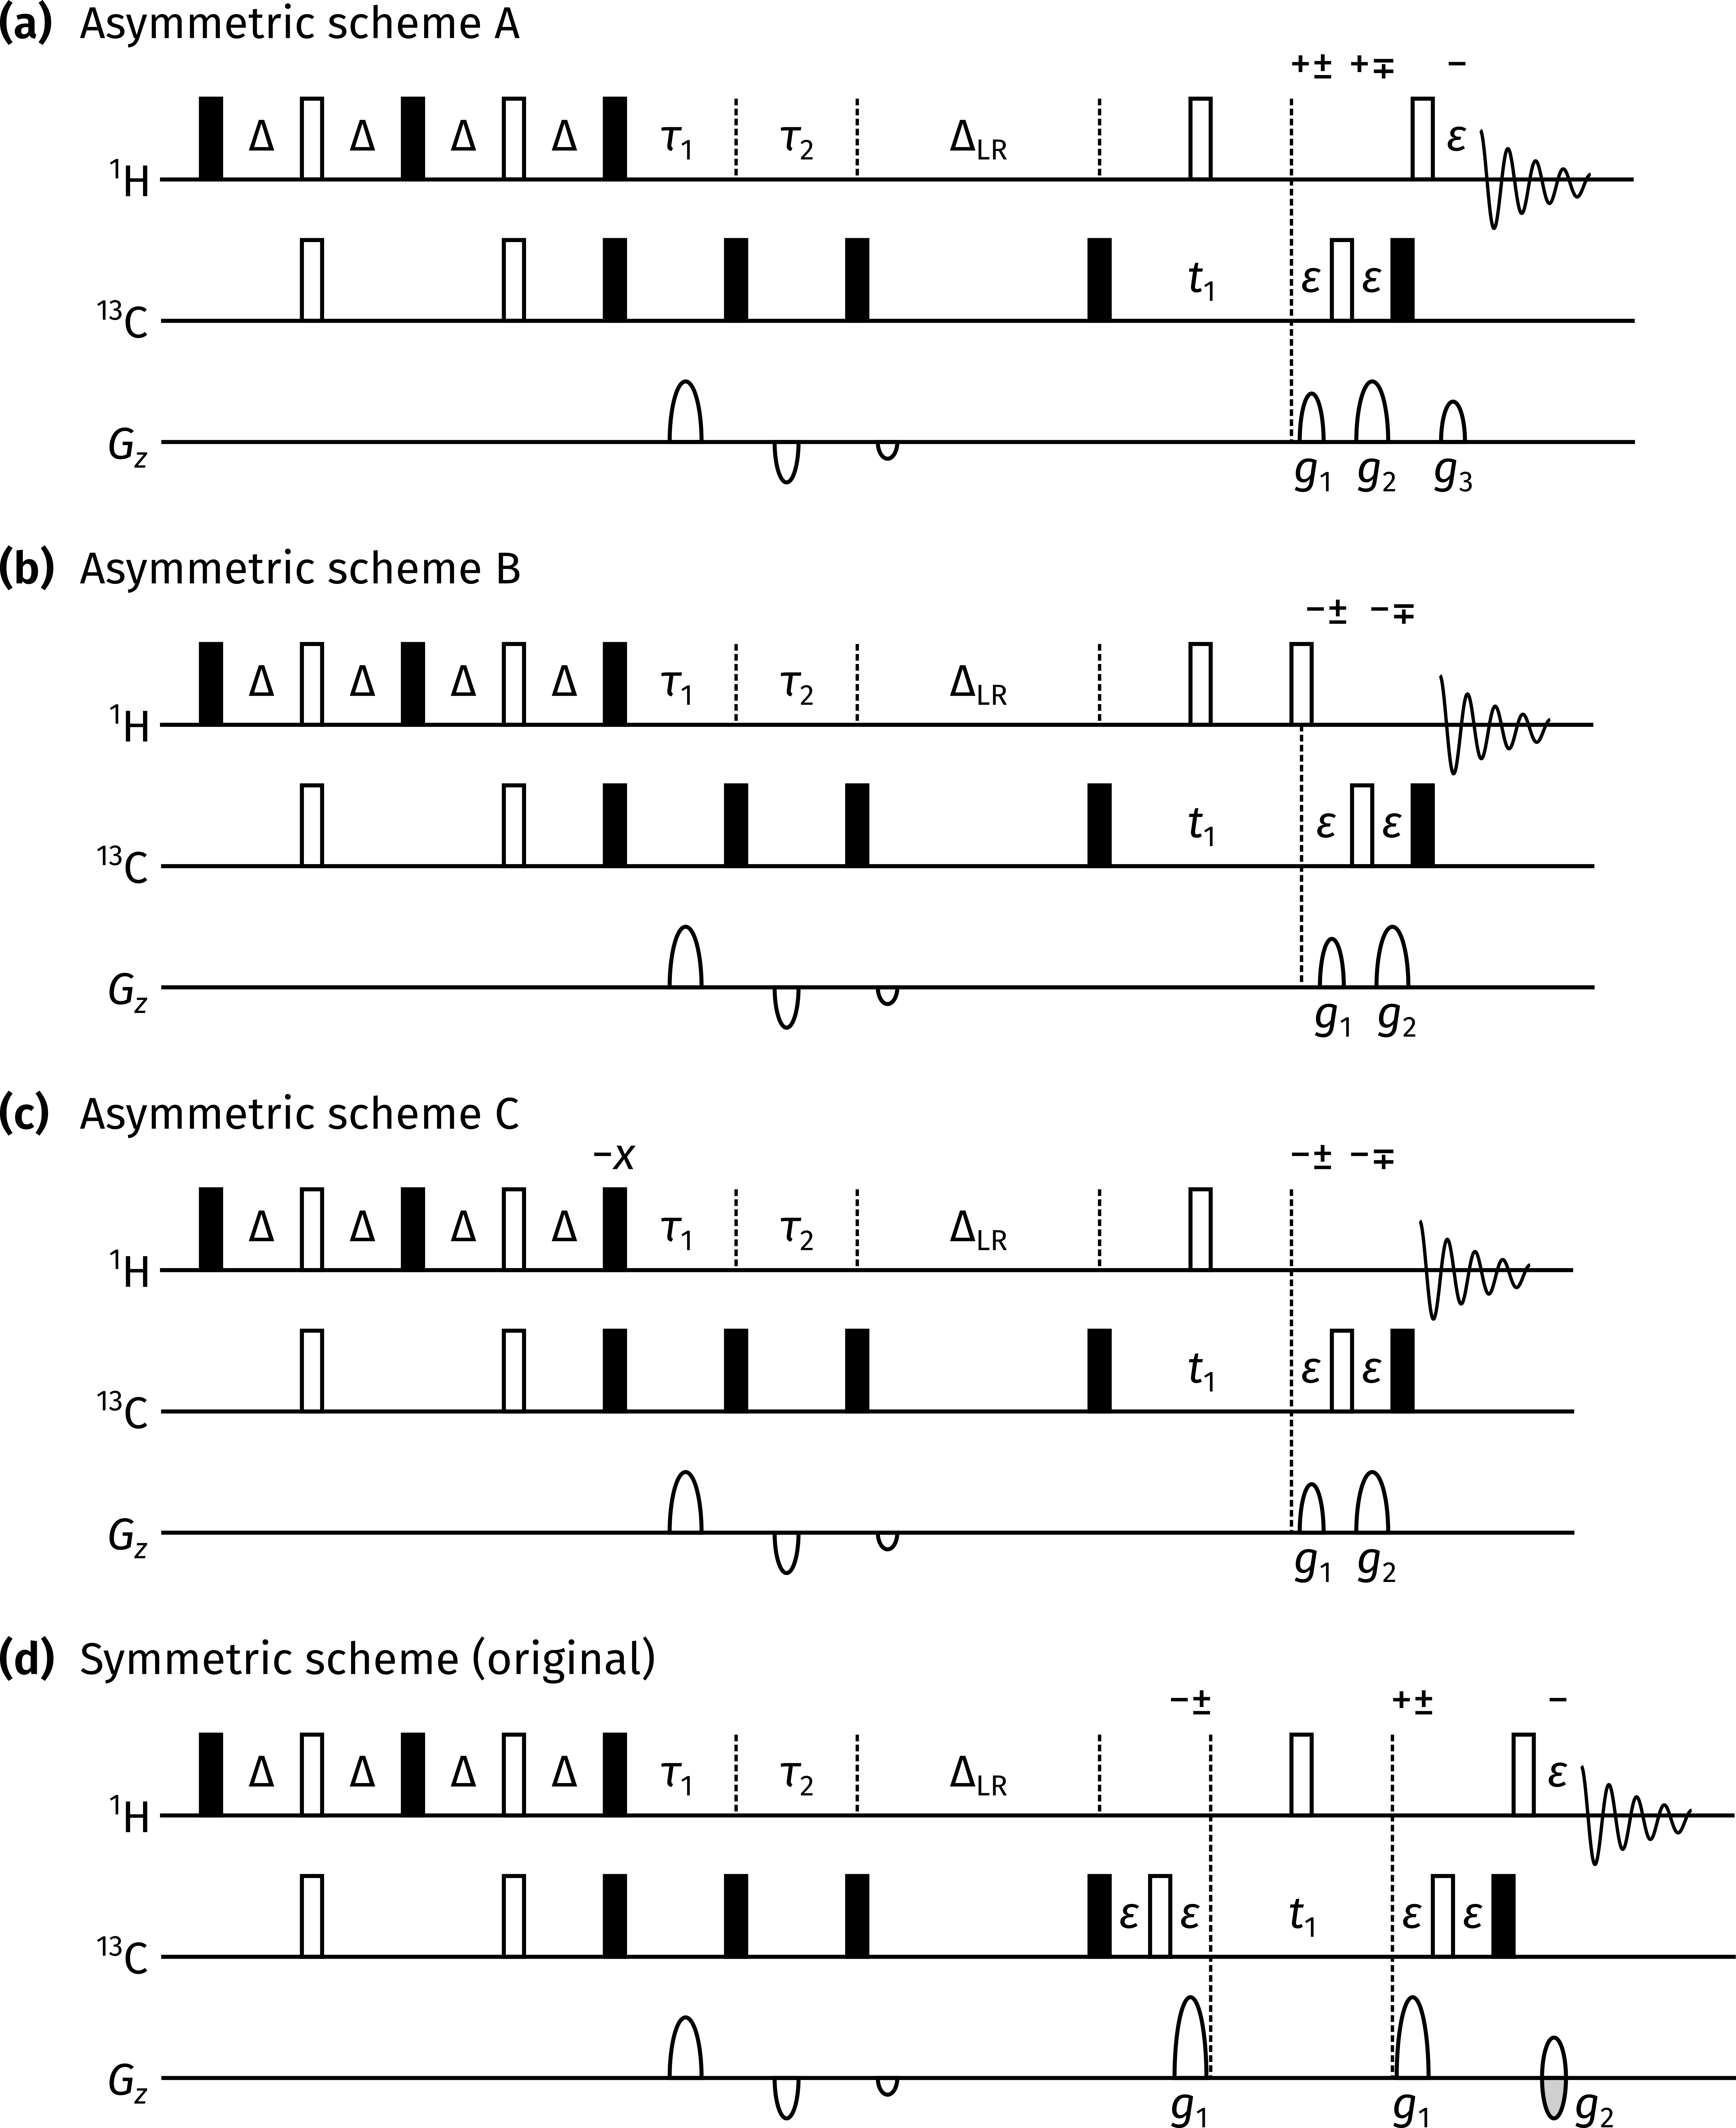
\includegraphics[]{pp/hmbc/noah_grads.png}%
    {\phantomsubcaption\label{fig:noah_hmbc_grads_bga}}%
    {\phantomsubcaption\label{fig:noah_hmbc_grads_bgb}}%
    {\phantomsubcaption\label{fig:noah_hmbc_grads_bgc}}%
    {\phantomsubcaption\label{fig:noah_hmbc_grads_b}}%
    \caption[Alternative CTP gradient schemes investigated for NOAH HMBC]{
        Alternative CTP gradient schemes investigated for the NOAH HMBC module.
        The coherences selected for during each gradient are indicated above each gradient, using the same notation for product operators as described in the \textit{Preface}: the `upper' term (e.g.\ $+$ in $\pm$) refers to the echo experiment, and the `lower' term to the antiecho experiment.
        So, for example, $+\pm$ refers to selection of $I_+S_+$ during the echo experiment and $I_+S_-$ during the antiecho experiment.
        Gradient amplitudes are as described in the text.
        \textbf{(\subref{fig:noah_hmbc_grads_bga})} `Asymmetric scheme A', modified from the standard library sequence to include an additional \ang{180} pulse and gradient.
        \textbf{(\subref{fig:noah_hmbc_grads_bgb})} `Asymmetric scheme B', where the \ang{180} pulse is shifted forward to the end of $t_1$.
        \textbf{(\subref{fig:noah_hmbc_grads_bgc})} `Asymmetric scheme C', which modifies the $zz$-filter instead of using an extra \ang{180} pulse.
        \textbf{(\subref{fig:noah_hmbc_grads_b})} The original `symmetric' scheme (the same as in \cref{fig:noah_sb_po_b}), placed here for convenience.
    }
    \label{fig:noah_hmbc_grads}
\end{figure}

Using this knowledge, it is possible to construct several `asymmetric' gradient schemes:
\begin{enumerate}
    \item `Scheme A' (\cref{fig:noah_hmbc_grads_bga}) is modified from the Bruker standard library to include a \ang{180} pulse and gradient at the end.
        The presence of an additional gradient means that there is a free parameter, here denoted as $\alpha$, which can be used to control the relative amplitudes of these three CTP gradients.
        The gradient amplitudes are chosen as follows:
        \begin{align}
            &\text{echo:}     & g_1 &= gc_1 & g_2 &= g    & g_3 &= gc_2 \label{eq:noah_hmbc_grads_bga_echo} \\
            &\text{antiecho:} & g_1 &= g    & g_2 &= gc_1 & g_3 &= gc_2 \label{eq:noah_hmbc_grads_bga_antiecho}
        \end{align}
        where $c_1 = -\alpha(\gammaH - \gammaC)/(\gammaH + \gammaC)$ and $c_2 = (1 - \alpha) (\gammaH - \gammaC)/\gammaH$.
        In principle $g$ is also a free parameter; for maximum suppression of artefacts I chose a relatively large value of 80\%.
    \item In `Scheme B' (\cref{fig:noah_hmbc_grads_bgb}), the \ang{180} pulse is shifted to immediately after $t_1$, before any of the CTP gradients have been applied. This means that there is no need for a third gradient, and the CTP gradient amplitudes can be directly taken from the standard library sequence:
        \begin{align}
            &\text{echo:}     & g_1 &= g  & g_2 &= gc \label{eq:noah_hmbc_grads_bgb_echo} \\
            &\text{antiecho:} & g_1 &= gc & g_2 &= g \label{eq:noah_hmbc_grads_bgb_antiecho}
        \end{align}
        where $c = -(\gammaH - \gammaC)/(\gammaH + \gammaC)$ and $g = 80\%$.
    \item `Scheme C' (\cref{fig:noah_hmbc_grads_bgc}) simply does not add a \ang{180} pulse, but instead modifies the phases of the $zz$-filter in order to place \magn{C} magnetisation along the $-z$ axis during the HMBC J-evolution delay.
        Here, the gradient amplitudes are the same as those in the standard library sequence as well as in scheme B.
\end{enumerate}

It is of interest to note two limiting cases of scheme A: when $\alpha = (\gammaH + \gammaC)/(\gammaH - \gammaC) \approx 1.67$, we have that $g_1 : g_2 : g_3 = 1 : -1 : \pm 2\gammaC/\gammaH$, which mimics the original `symmetric' scheme (\cref{fig:noah_hmbc_grads_b}); and when $\alpha = 1$, we have that $g_3 = 0$, i.e.\ a return to the two-gradient tactic of schemes B and C.
In the tests which follow, I ran scheme A with $\alpha = 1.67$, $\alpha = 0.6$, and $\alpha = 0.3$.

\begin{figure}[htb]
    \centering
    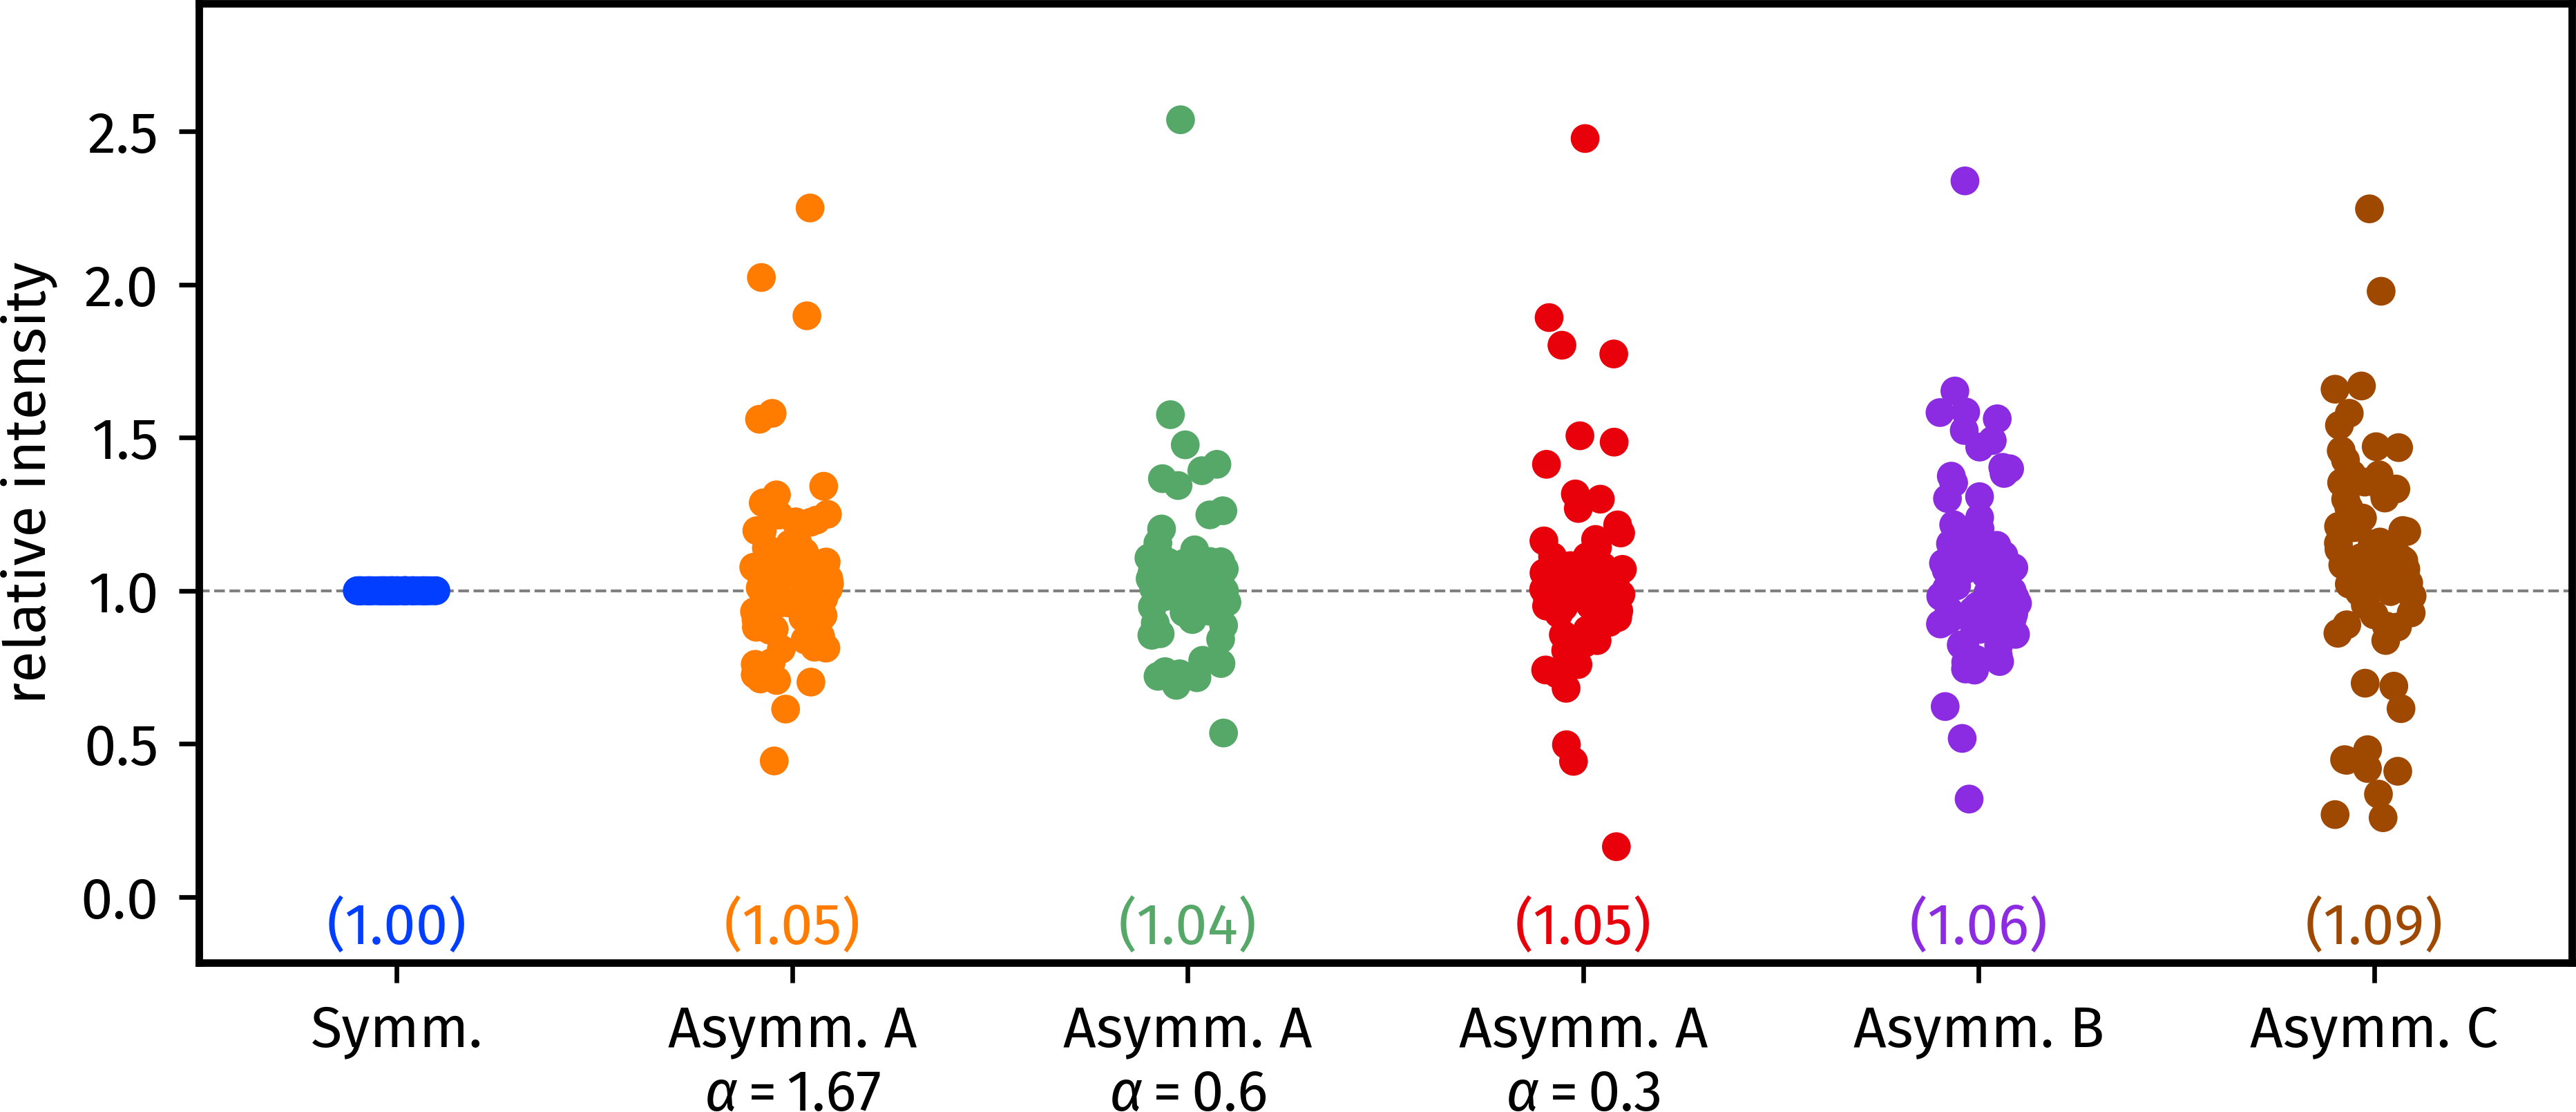
\includegraphics[]{noah/hmbc_grad_sens.png}%
    \caption[Comparison of relative sensitivities of HMBC gradient schemes]{
        Sensitivities of various asymmetric HMBC gradient schemes, as compared to the symmetric scheme in \cref{fig:noah_sb_po_b}.
        Each dot indicates one crosspeak in the HMBC spectrum; the numbers in parentheses are the average over all peaks.
        \datacode{7A-211226}
    }
    \label{fig:hmbc_grad_sens}
\end{figure}

All of the different HMBC versions above, plus the original `symmetric' scheme in \cref{fig:noah_sb_po_b}, were tested in the context of a \noah{B,S} supersequence using the andrographolide sample (\cref{fig:hmbc_grad_sens}).
Since the HMBC module is the first module in this supersequence, the values here are an accurate reflection of their intrinsic sensitivities.
As can be seen, there is not much at all which separates the different versions (outliers with $>2\times$ `sensitivity improvements' can be attributed to different J-modulation in the multiplet).
The most sensitive of these is asymmetric scheme C, which may be explained by the fact that it has one fewer \ang{180} pulse: however, this comes with an immediate drawback.
Since scheme C places the \magn{C} magnetisation along $-z$ during the LPJF as well as the J-evolution delay $\Delta_\text{LR}$ (a total of ca.\ \qty{70}{\ms}), relaxation losses during this period lead to poorer retention of \magn{C} magnetisation for later modules, as shown by the decreased HSQC sensitivities in \cref{fig:hmbc_grad_sens_hsqc}.
In contrast, all the other gradient schemes retain \magn{C} magnetisation equally well.

\begin{figure}[htb]
    \centering
    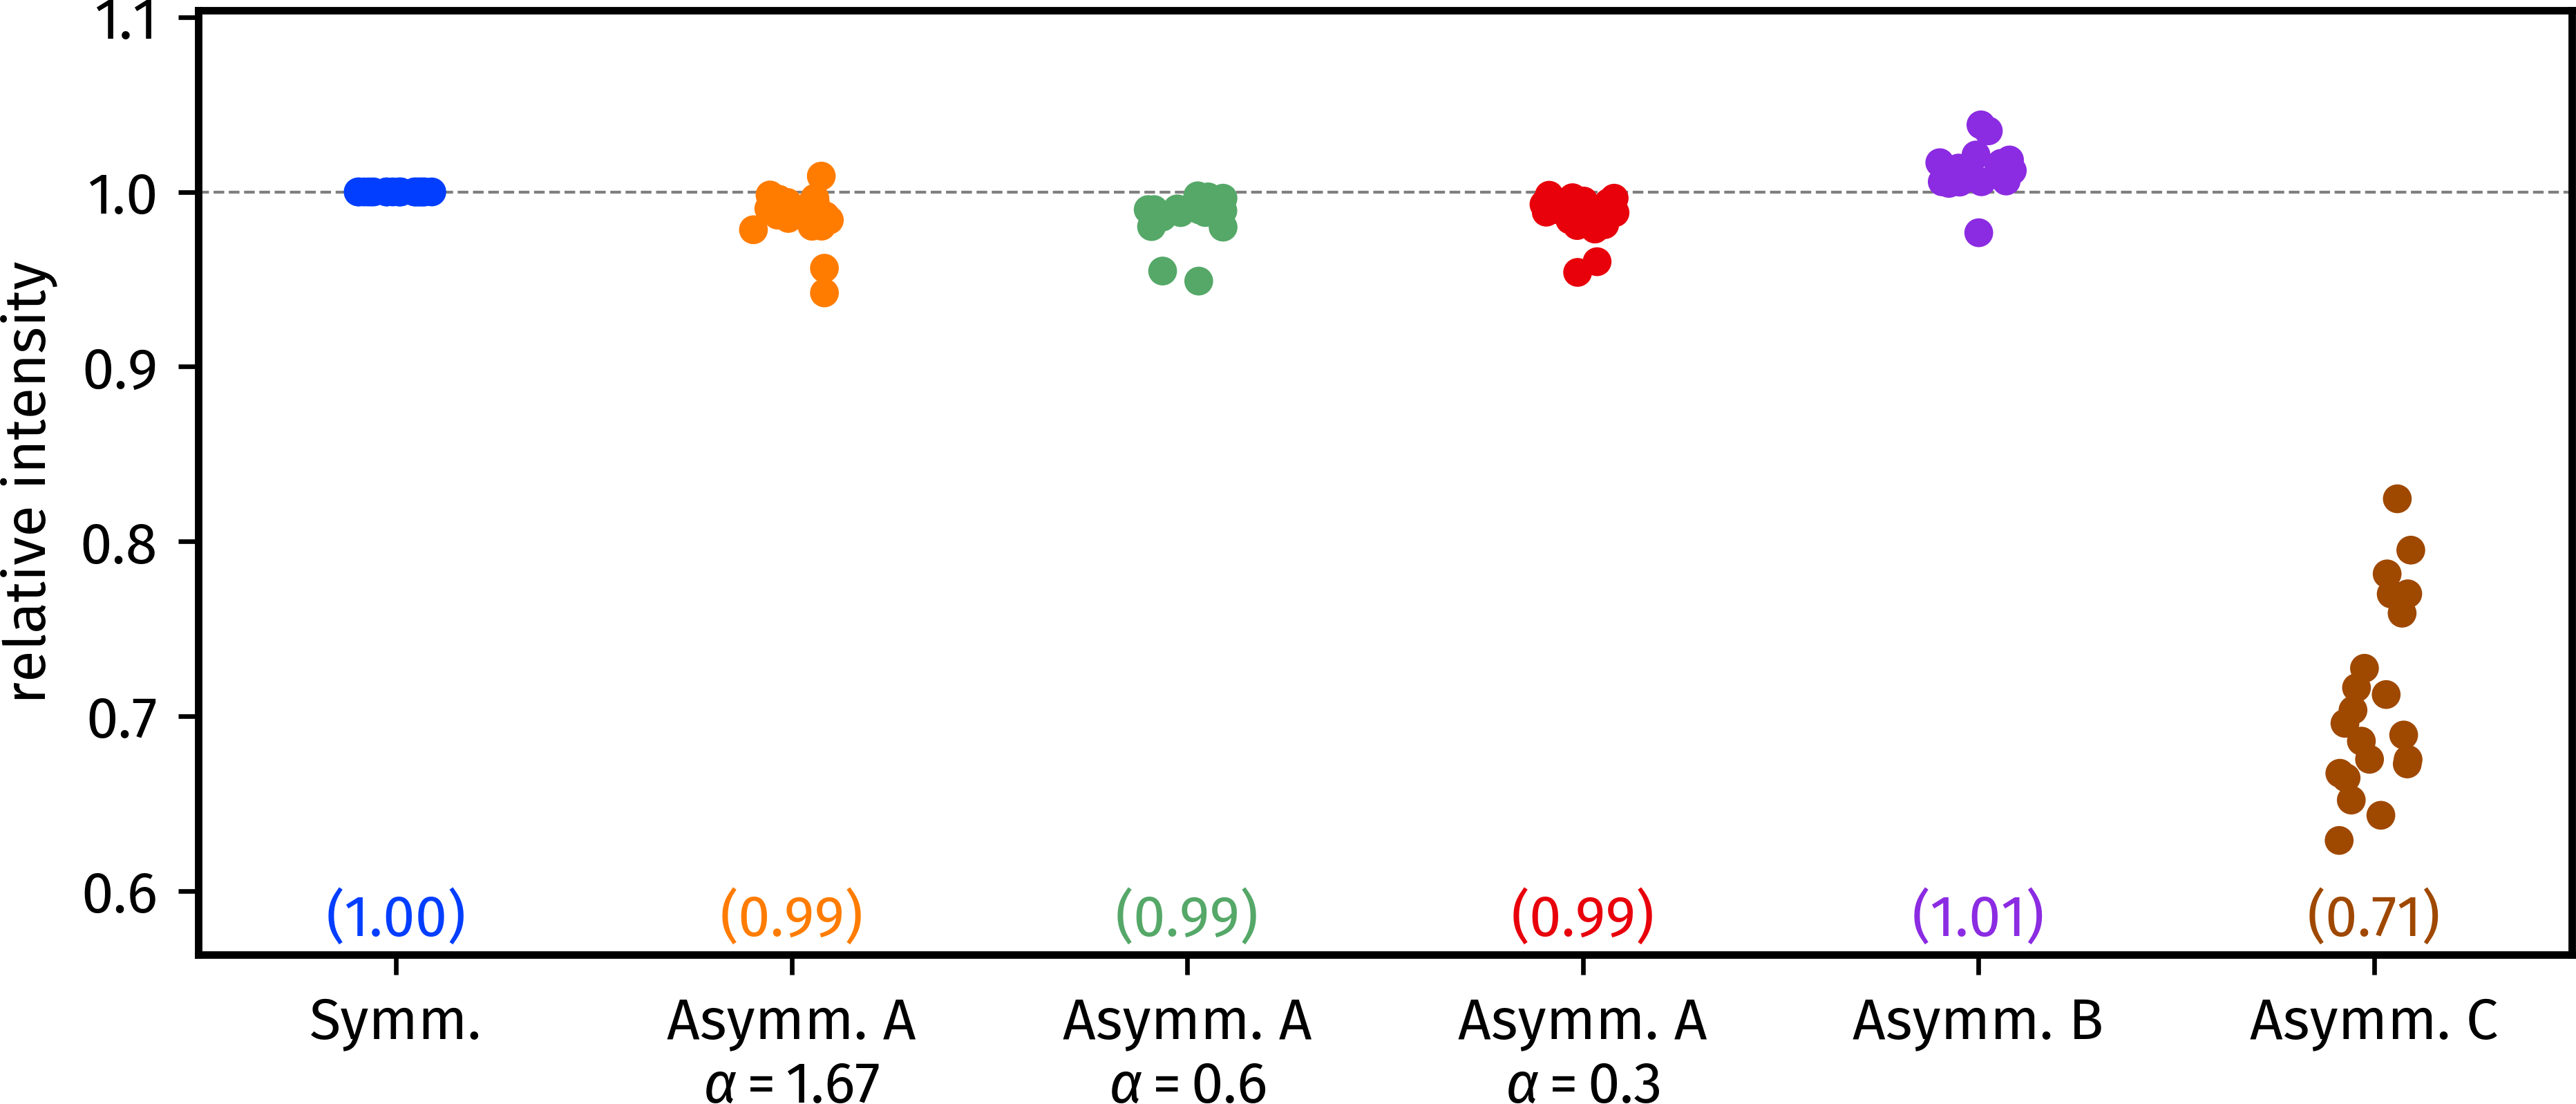
\includegraphics[]{noah/hmbc_grad_sens_hsqc.png}%
    \caption[Effect of HMBC gradient scheme on HSQC sensitivity in a \noah{B,S} supersequence]{
        Sensitivities of the HSQC module in a \noah{B,S} supersequence, where the HMBC module is implemented using the gradient schemes of \cref{fig:hmbc_grad_sens}.
        \datacode{7A-211226}
    }
    \label{fig:hmbc_grad_sens_hsqc}
\end{figure}

The final point worth studying is the quality of the HMBC spectrum itself.
To do this, we need to look at the actual spectra (\cref{fig:hmbc_grad_spec}).
For the most part, the spectra are all the same; however, there is a notable set of artefacts present in \cref{fig:hmbc_grad_spec_asymma1} (scheme A with $\alpha = 1.67$) as well as \cref{fig:hmbc_grad_spec_asymmb} (scheme B), highlighted in red boxes.
These artefacts occur at the frequencies
\begin{equation}
    \label{eq:hmbc_wing_artefacts}
    (\Omega_1, \Omega_2) = \left(\Omega_S \pm \frac{\Omega_I}{2}, \Omega_I\right),
\end{equation}
and are in fact `wing' artefacts similar to that observed in other modules \todo{insert reference}.
In this case, they arise due to imperfect refocusing of the \proton{} chemical shift during $t_1$: specifically, whenever $I_zS_\pm$ terms are present during the second half of $t_1$.
Extra evidence for the origin of these artefacts comes from the observation that when the \ang{180} pulse in the middle of $t_1$ is phase cycled, the artefacts are removed.
In a standard HMBC, these terms would not be detected in the final FID; however, in this case, the addition of an extra \ang{180} pulse after $t_1$ provides an opportunity for these to be converted back into observable spin-$I\/$ magnetisation (through off-resonance effects or miscalibration).

The poorer performance may therefore be understood as follows:
when scheme A is acquired with $\alpha = 1.67$, the gradients $g_1$ and $g_2$ have equal and opposite amplitudes, and so do not enforce any coherence selection on spin $I\/$ during the second half of $t_1$.
Likewise, scheme B contains no gradients during the second half of $t_1$.

\begin{figure}[htb]
    \centering
    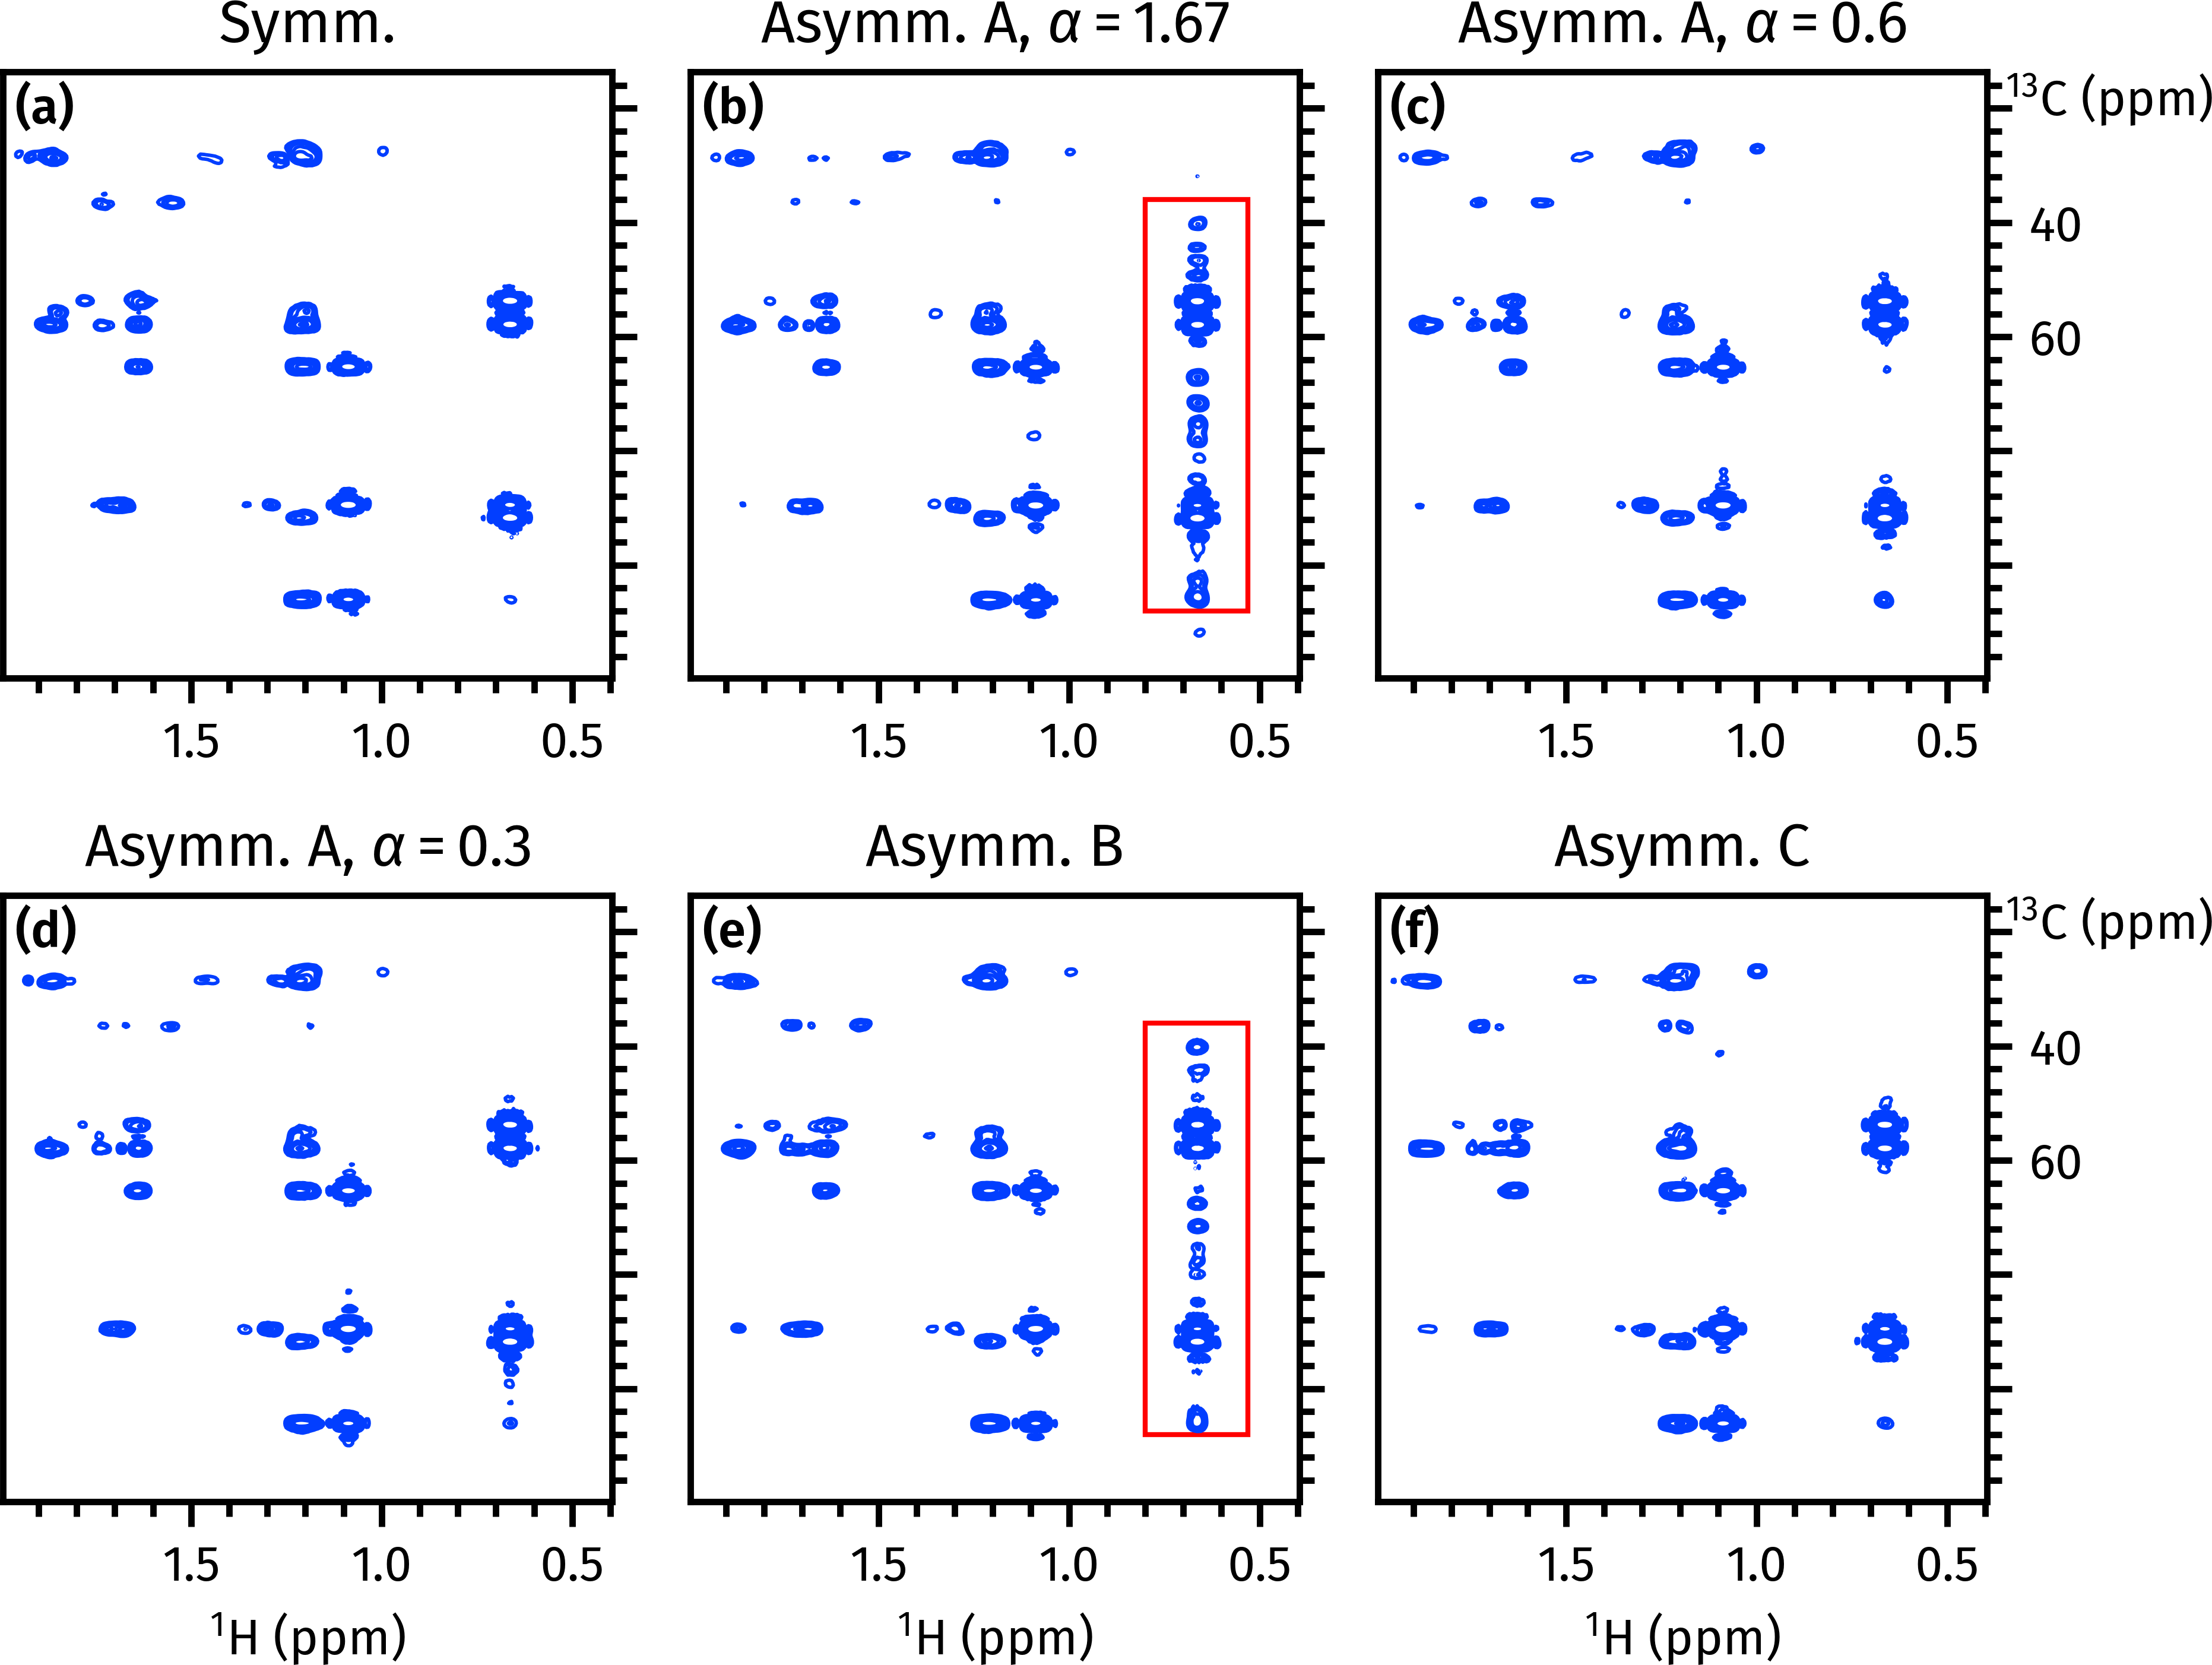
\includegraphics[]{noah/hmbc_grad_spec.png}%
    {\phantomsubcaption\label{fig:hmbc_grad_spec_symm}}%
    {\phantomsubcaption\label{fig:hmbc_grad_spec_asymma1}}%
    {\phantomsubcaption\label{fig:hmbc_grad_spec_asymma2}}%
    {\phantomsubcaption\label{fig:hmbc_grad_spec_asymma3}}%
    {\phantomsubcaption\label{fig:hmbc_grad_spec_asymmb}}%
    {\phantomsubcaption\label{fig:hmbc_grad_spec_asymmc}}%
    \caption[HMBC spectra acquired with different gradient schemes]{
        HMBC spectra acquired with the gradient schemes of \cref{fig:hmbc_grad_sens}.
        Extra `wing' artefacts present in two of the spectra (asymmetric scheme A with $\alpha = 1.67$, \textbf{(\subref{fig:hmbc_grad_spec_asymma1})}, and asymmetric scheme B, \textbf{(\subref{fig:hmbc_grad_spec_asymmb})}) are highlighted in red boxes.
    }
    \label{fig:hmbc_grad_spec}
\end{figure}

The characteristics of these gradient schemes are summarised in \cref{tbl:hmbc_grads}.
As can be seen, the `best' schemes are either the original symmetric scheme, or asymmetric scheme A with $\alpha \neq 1.67$.
However, there is not much difference between these: it is not clear whether the improvement in sensitivity is reproducible across a wide range of samples, and in any case, the gains are extremely marginal.

\begin{table}[htb]
    \begin{tabular}{cccc}
        \toprule
        \textbf{Gradient scheme} & \textbf{HMBC sensitivity} & \textbf{HSQC sensitivity} & \textbf{Wing artefacts} \\
        \midrule
        Symmetric                     & 1    & 1    & No  \\
        Asymmetric A, $\alpha = 1.67$ & 1.05 & 0.99 & Yes \\
        Asymmetric A, $\alpha = 0.6$  & 1.04 & 0.99 & No  \\
        Asymmetric A, $\alpha = 0.3$  & 1.05 & 0.99 & No  \\
        Asymmetric B                  & 1.06 & 1.01 & Yes \\
        Asymmetric C                  & 1.09 & 0.71 & No  \\
        \bottomrule
    \end{tabular}
    \caption[Comparison of HMBC gradient schemes]{
        Comparison of HMBC gradient schemes discussed in this section: the data are a summary of \cref{fig:hmbc_grad_sens,fig:hmbc_grad_sens_hsqc,fig:hmbc_grad_spec}.
    }
    \label{tbl:hmbc_grads}
\end{table}


\subsubsection{Other artefacts}

It has been established that the HMBC module (and supersequences containing it) are not fully ideal in terms of magnetisation preservation.
However, there are also some other curious phenomena which have not been fully described in the literature.
One of these is the presence of \textit{inverted peaks} in the homonuclear X module(s) in a \noah{B,S,X} supersequence: this is illustrated in \cref{fig:hmbc_invert_1_orig} with the CLIP-COSY module (\noah*{X} = \noah*{Cc}).
It is not clear why this occurs, because the HMBC module (and the gradients which follow) should dephase all \magnnot{C} magnetisation.
Although this leads to reduced sensitivity in the homonuclear module, in that the signal derives from polarisation which has recovered during the preceding FIDs, it is not clear why this polarisation should be \textit{negative}.
One clue lies in the fact that these peaks are very sensitive to the \proton{} \ang{90} pulse width: simply changing this by \qty{0.5}{\us} is sufficient to restore the correct signal sign (\cref{fig:hmbc_invert_1_pw}).

\begin{figure}[htb]
    \centering
    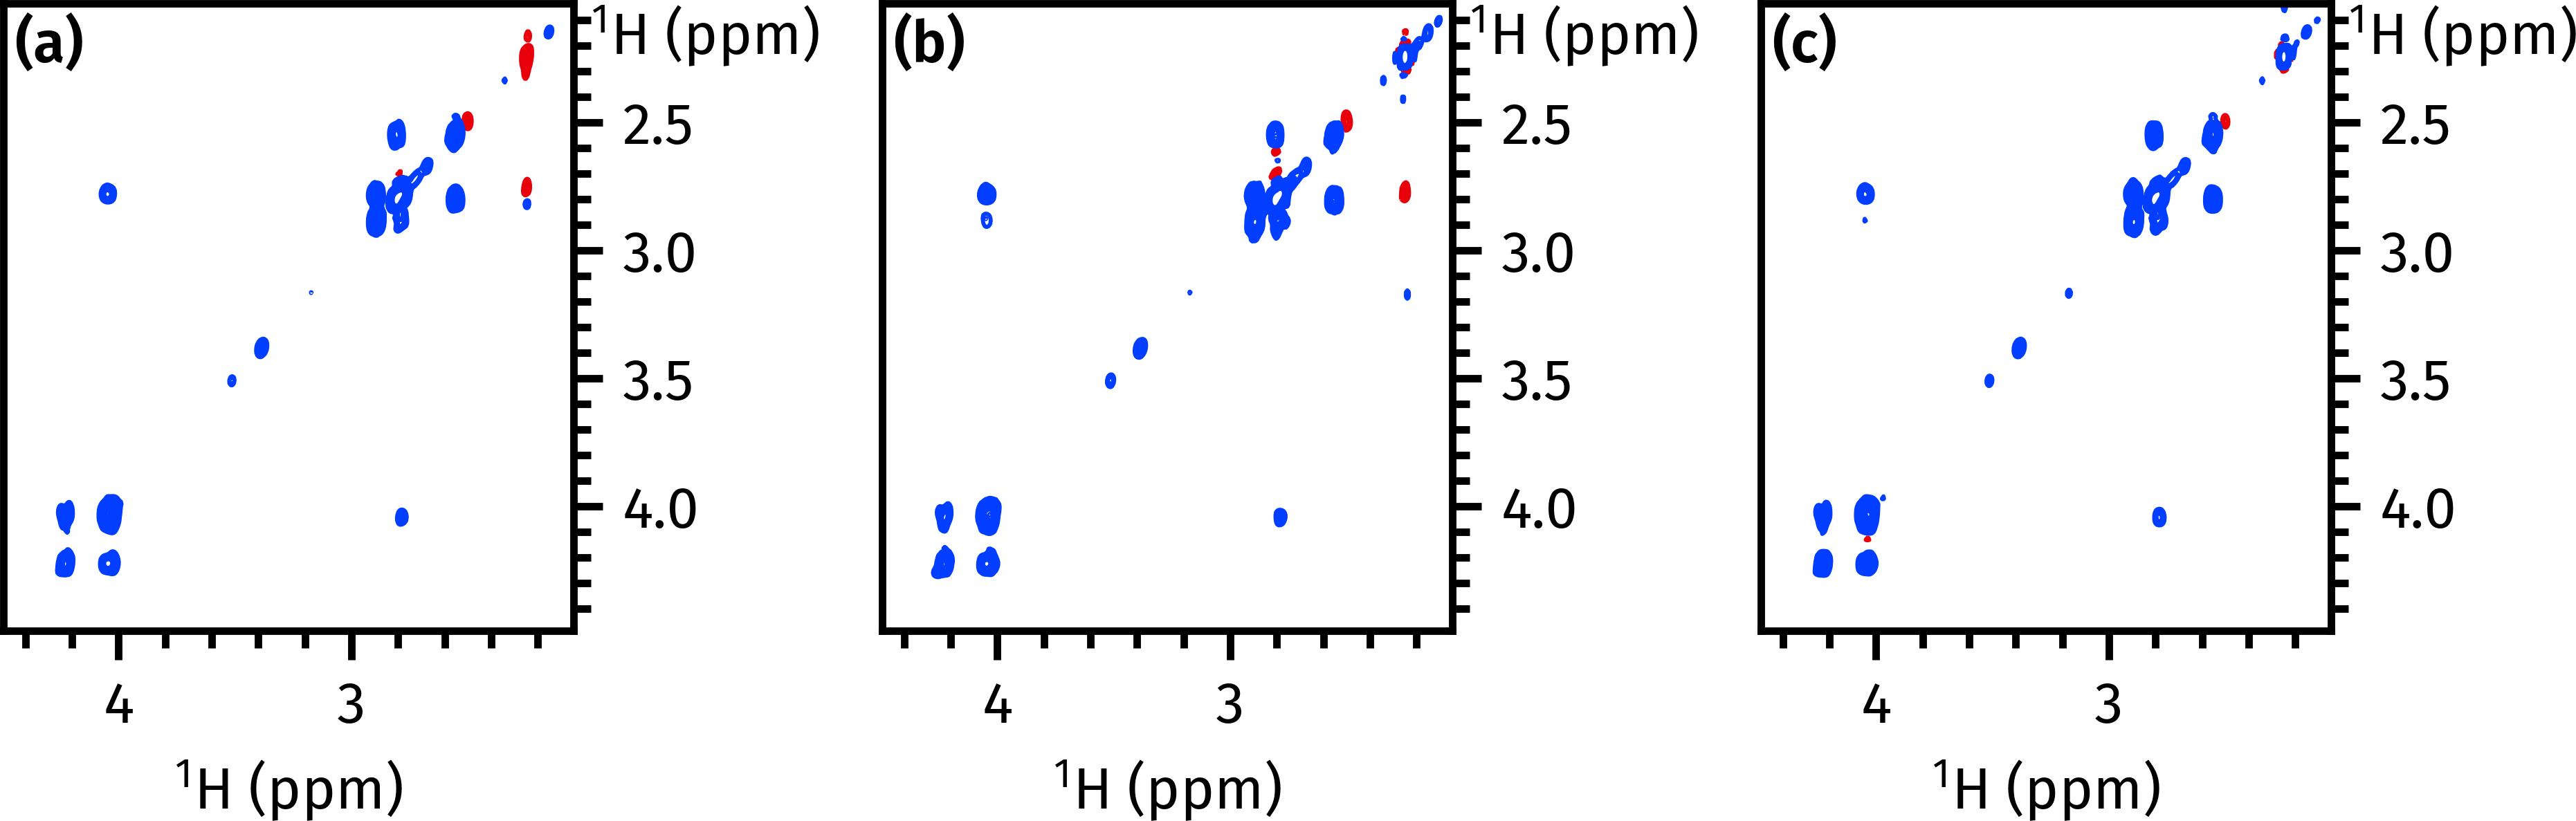
\includegraphics[]{noah/hmbc_invert_1.png}%
    {\phantomsubcaption\label{fig:hmbc_invert_1_orig}}%
    {\phantomsubcaption\label{fig:hmbc_invert_1_pw}}%
    {\phantomsubcaption\label{fig:hmbc_invert_1_bssc}}%
    \caption[Inverted peaks in homonuclear module of \noah*{B,S,X}-type supersequences]{
        \textbf{(\subref{fig:hmbc_invert_1_orig})} CLIP-COSY from a \noah{B,S,Cc} supersequence, acquired with a \proton{} \ang{90} pulse width of \qty{11.28}{\us} (this value was obtained using the POISE calibration described in \cref{subsec:poise__pulsecal}).
        An inverted peak is visible at \qty{2.25}{\ppm}.
        \textbf{(\subref{fig:hmbc_invert_1_pw})} The same, but acquired using a \ang{90} pulse width of \qty{11.78}{\us}.
        \textbf{(\subref{fig:hmbc_invert_1_bssc})} CLIP-COSY from a \noah{B,S,S,Cc} supersequence. The \ang{90} pulse width was \qty{11.28}{\us}, the same as in (\subref{fig:hmbc_invert_1_orig}).
        \datacode{7Z-220214}
    }
    \label{fig:hmbc_invert_1}
\end{figure}

The modules placed between the HMBC and the homonuclear module also play an important role.
When \textit{two} HSQC modules are used, i.e.\ a \noah{B,S,S,Cc} supersequence (using $f = 0.7$ as described in \cref{subsec:noah__hsqctocsy}---although this is unlikely to matter), the negative peaks are no longer observed (\cref{fig:hmbc_invert_1_bssc}).
In fact, having \textit{no modules} between the HMBC and the homonuclear module is also (at least sometimes) acceptable: a separate set of data shows that the inverted peaks in an \noah{B,Sp,Cc} experiment are not seen in a \noah{Sp,B,Cc} supersequence (\cref{fig:hmbc_invert_2_bspc,fig:hmbc_invert_2_spbc}).
The use of ASAP mixing just before the homonuclear module does not remedy this (\cref{fig:hmbc_invert_2_bspc_asap,fig:hmbc_invert_2_spbc_asap}).
Unfortunately, a good explanation for these artefacts has remained elusive.

\begin{figure}[!ht]
    \centering
    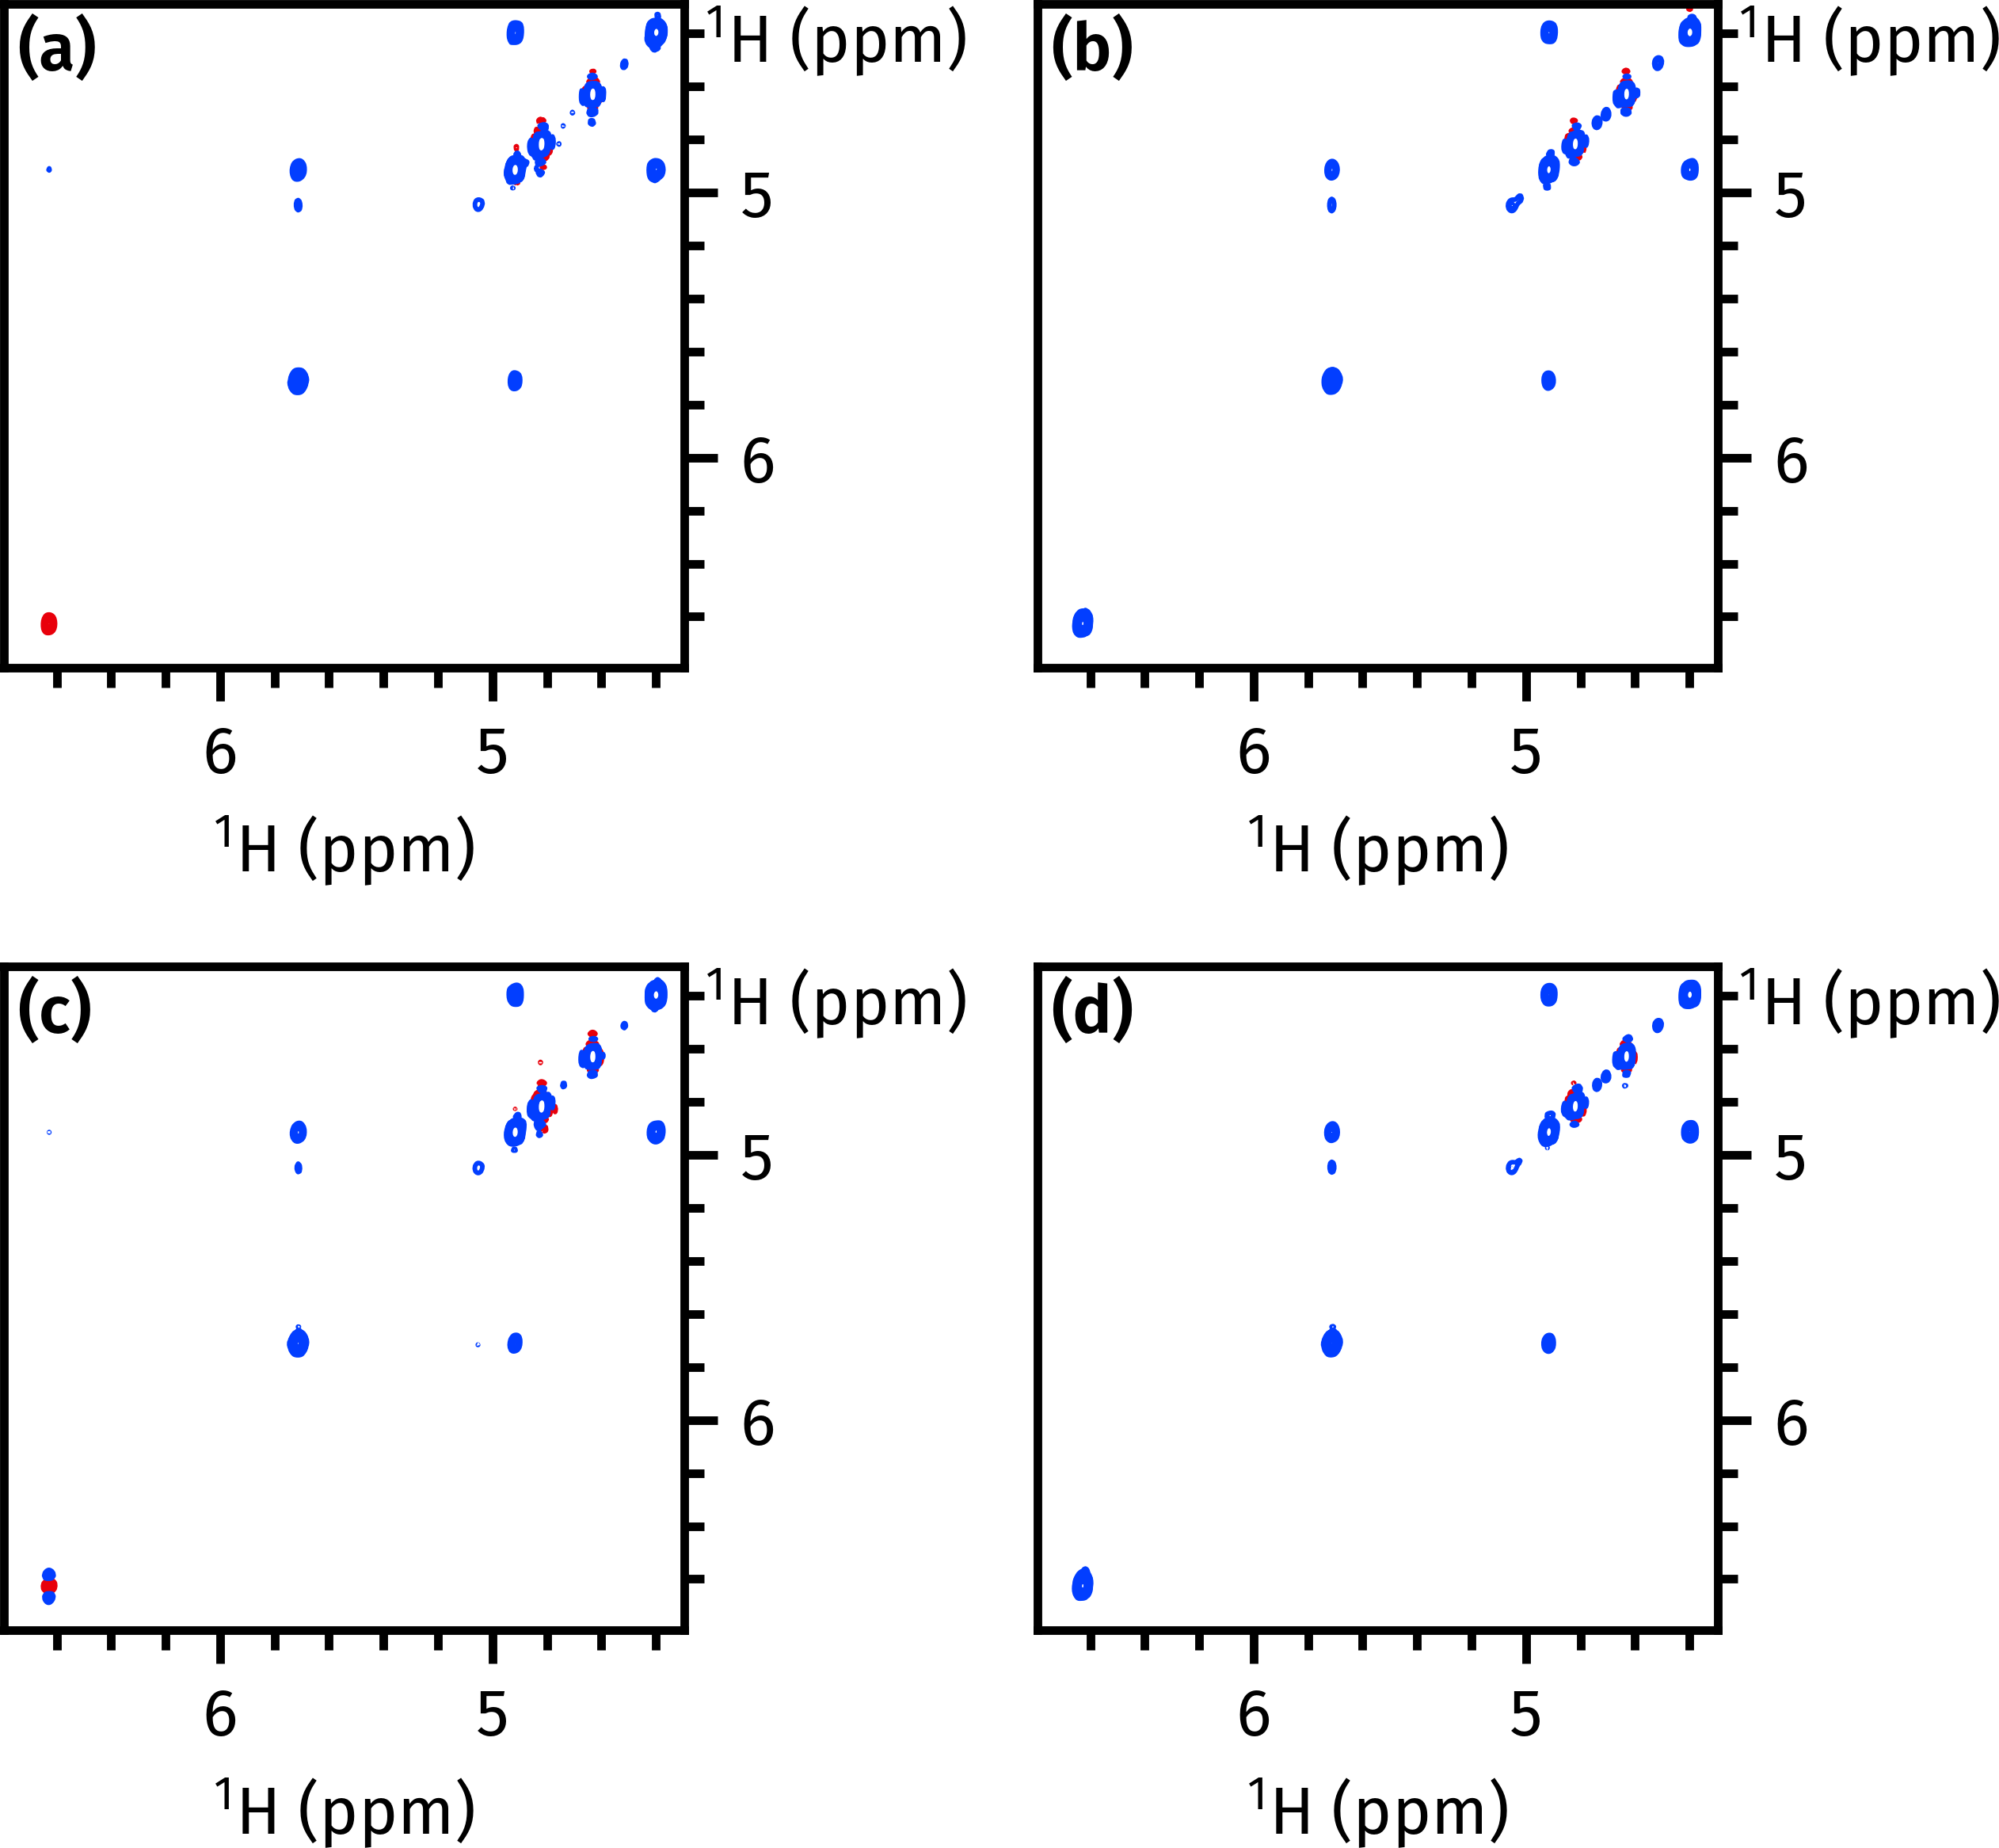
\includegraphics[]{noah/hmbc_invert_2.png}%
    {\phantomsubcaption\label{fig:hmbc_invert_2_bspc}}%
    {\phantomsubcaption\label{fig:hmbc_invert_2_spbc}}%
    {\phantomsubcaption\label{fig:hmbc_invert_2_bspc_asap}}%
    {\phantomsubcaption\label{fig:hmbc_invert_2_spbc_asap}}%
    \caption[Effect of module ordering and ASAP mixing on inverted peaks in \noah*{B,S,X}-type supersequences]{
        \textbf{(\subref{fig:hmbc_invert_2_bspc})} CLIP-COSY from a \noah{B,Sp,Cc} supersequence.
        An inverted diagonal peak can be seen at \qty{6.6}{\ppm}.
        \textbf{(\subref{fig:hmbc_invert_2_spbc})} From a \noah{Sp,B,Cc} supersequence.
        \textbf{(\subref{fig:hmbc_invert_2_bspc_asap})--(\subref{fig:hmbc_invert_2_spbc_asap})} The same as (\subref{fig:hmbc_invert_2_bspc}) and (\subref{fig:hmbc_invert_2_spbc}), but with \qty{40}{\ms} ASAP mixing placed just before the CLIP-COSY module.
        \datacode{7A-211227}
    }
    \label{fig:hmbc_invert_2}
\end{figure}

\subsubsection{\nitrogen{} HMBC module}

The entirety of this section has---until now---been devoted to the \carbon{} HMBC module.
However, the techniques used in constructing this, including the implementation of the $zz$-filter, are equally applicable to a \nitrogen{} HMBC.
For simplicity, the NOAH \nitrogen{} HMBC module uses a first-order LPJF (since $\oneJ{NH}$ pairs are less common); this may be omitted if desired.
To minimise the number of pulses, a simple magnitude-mode version of the HMBC is used (\cref{fig:noah_15n_hmbc}).
The implementation of this module within supersequences is discussed in greater detail within the context of \textit{generalised supersequences}, in \todo{REF}.

\begin{figure}[htb]
    \centering
    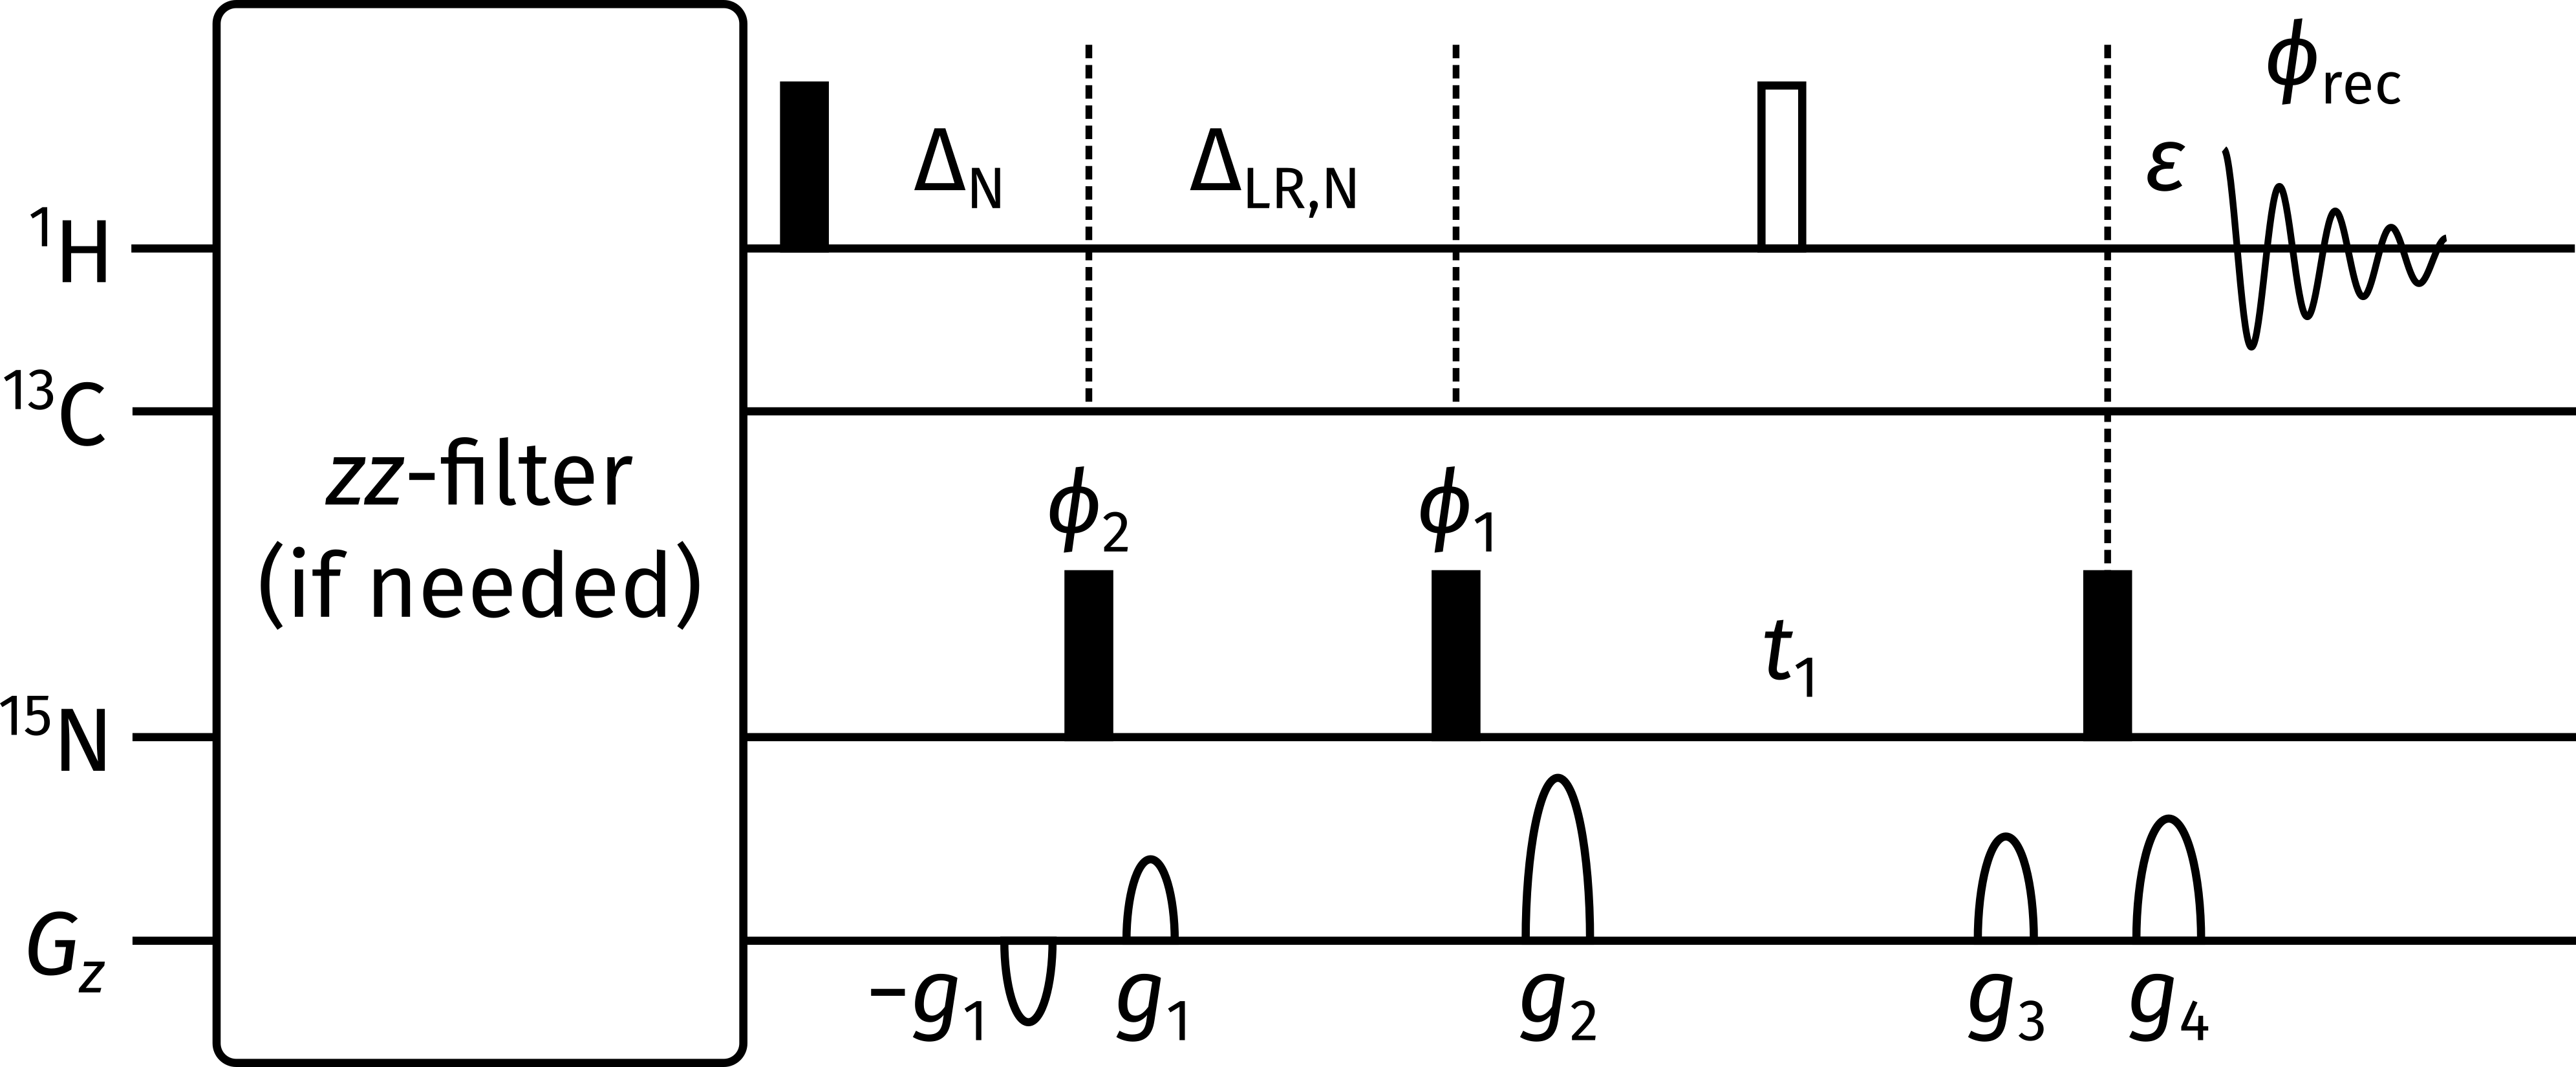
\includegraphics[]{pp/hmbc_15n.png}%
    \caption[NOAH \nitrogen{} HMBC module]{
        NOAH \nitrogen{} HMBC module.
        The $zz$-filter can be implemented as necessary in the same way as for the \carbon{} HMBC module (a final \proton{} \ang{180} pulse may also be required, but is not shown here).
        Delays are set as follows: $\Delta_{\ch{N}} = 1 / (2 \cdot \oneJ{NH})$; $\Delta_{\text{LR},\ch{N}} = 1 / (2 \cdot \nJ{NH})$.
        Phase cycling is performed using $\phi_1 = \phi_\text{rec} = (x, -x)$ and $\phi_2 = (x, x, -x, -x)$.
        Gradient amplitudes are $(g_1, g_2, g_3, g_4) = (5\%, 70\%, 30\%, 50.1\%)$.
    }
    \label{fig:noah_15n_hmbc}
\end{figure}
